\documentclass[12pt,letterpaper]{hmcpset}
\usepackage[margin=1in]{geometry}
\usepackage{graphicx}
\usepackage[makeroom]{cancel}
\usepackage{array}
\usepackage{mathtools}
\usepackage{marginnote}
\usepackage{units}
\usepackage{xfrac}
\usepackage{enumerate}
\usepackage{amsmath}
\usepackage{fancyhdr}
\usepackage{pgfplots}
\usepackage{hyperref}
\usepackage{nopageno}
\usepackage{boondox-cal}
\hypersetup{
	colorlinks=true,
	linkcolor=blue,
	filecolor=magenta,
	urlcolor=magenta,
}

% info for header block in upper right hand corner
\name{} %put your name here
\class{Physics 51 Section \hspace{3mm}} %put your section here
\assignment{Homework 8}
\duedate{Monday, October 19, 2020}

\begin{document}
	\begin{problem}[SUP 8.1:]
		The design of some electronic devices can involve circuit boards with broad conducting copper planes, in addition to the usual use of narrow wires.
		Two such adjacent planes can be a source of inadvertent inductance in a circuit.
		We will approximate this effect by considering two large, thin parallel conducting plates situated a distance $d$ apart, and carrying a current $I$ in parallel but opposite directions.
		Let the width $w$ and the length $h$ parallel to the direction of current flow be much larger than $d$, so that edge fringing effects may be neglected.
		(Let the plates have vanishingly small thickness.)

		\

		\centering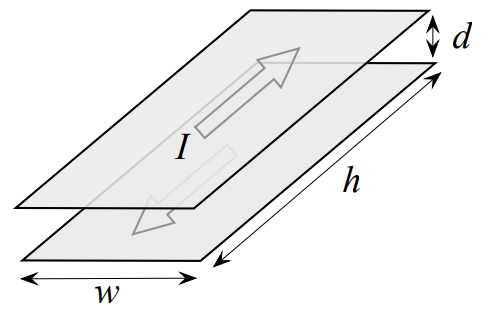
\includegraphics[scale = 0.6]{Sup_8-1}
		
		\begin{enumerate}[(a)]
			\item Determine the magnetic field $\vec{\mathbf{B}}$ everywhere due to this configuration of current.
			\item Use the method of flux linkage to find the effective inductance of the two plates.
			\item Verify the answer to part (b) by using the method of energy storage.
		\end{enumerate}
	\end{problem}
	\clearpage



	\begin{problem}[36P3:]
		Two long, parallel wires, each of radius $a$, whose centers are a distance $d$ apart carry equal currents in opposite directions.
		Show that, neglecting the flux within the wires themselves, the inductance of a length $l$ of such a pair of wires is given by
		\[L = \frac{\mu_0l}{\pi}\ln{\frac{d - a}{a}}.\]
		See Sample Problem 33-4. (Hint: Calculate the flux through a rectangle of which the wires form two opposite sides.)
	\end{problem}
	\clearpage



	\begin{problem}[36P9:]
		\begin{enumerate}[(a)]
			\item Find an expression for the energy density as a function of the radial distance $r$ for a toroid of rectangular cross section.
			\item Integrating the energy density over the volume of the toroid, calculate the total energy stored in the field of the toroid.
			\item Using
			\[L = \frac{N\Phi_B}{i} = \frac{\mu_0N^2h}{2\pi}\ln{\frac{b}{a}},\]
			evaluate the energy stored in the toroid directly from the inductance and compare with (b).
		\end{enumerate}
	\end{problem}
	\clearpage



	\begin{problem}[36E44:]
		In the circuit shown in Fig. 36-22, the switch has been in position $a$ for a long time.
		It is now thrown to $b$.
		\begin{enumerate}[(a)]
			\item Calculate the frequency of the resulting oscillating current.
			\item What will be the amplitude of the current oscillations?
		\end{enumerate}
		
		\centering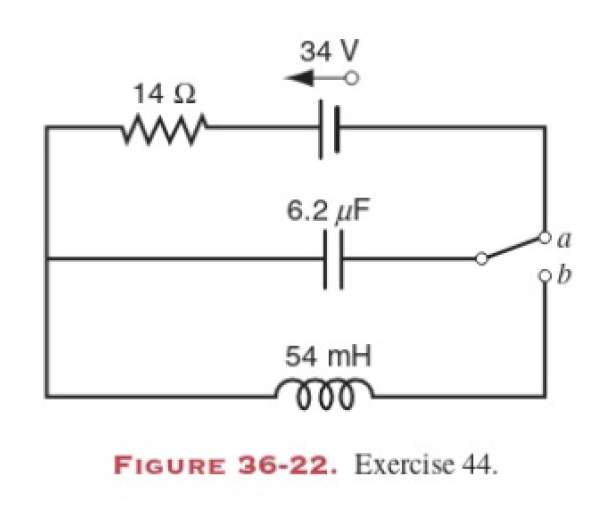
\includegraphics[scale = 0.4]{Fig_36-22}
	\end{problem}
	\clearpage



	\begin{problem}[38P3:]
		The capacitor in Fig. 38-25 consisting of two circular plates with radius $R$ = 18.2 cm is connected to a source of emf $\mathcal{E} = \mathcal{E}_m\sin{\omega t}$, where $\mathcal{E}_m$ = 225 V and $\omega$ = 128 rad/s.
		The maximum value of the displacement current is $i_d$ = 7.63 $\mu$A.
		Neglecting fringing of the electric field at the edges of the plates:
		\begin{enumerate}[(a)]
			\item What is the maximum value of the current $i$?
			\item What is the maximum value of $\frac{d\Phi_E}{dt}$, where $\Phi_E$ is the electric flux through the region between the plates?
			\item What is the separation $d$ between the plates?
			\item Find the maximum value of the magnitude of $\vec{\mathbf{B}}$ between the plates at a distance $r$ = 11.0 cm from the center.

			\centering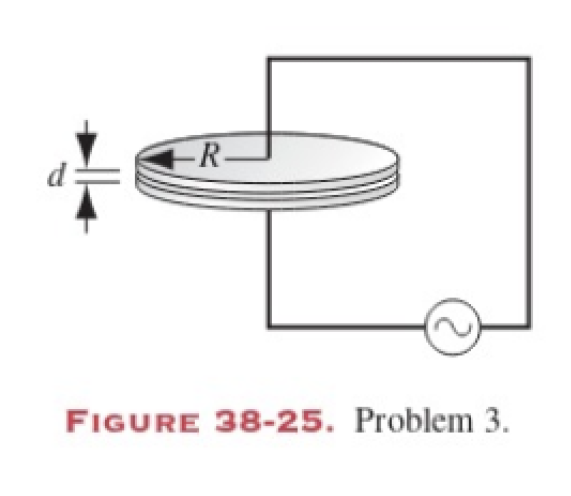
\includegraphics[scale = 0.4]{Fig_38-25}
		\end{enumerate}
	\end{problem}
	\clearpage



	\begin{problem}[SUP 8.2:]
		A parallel plate capacitor has circular plates of radius $R$ and separation $d$.
		The capacitor is connected to a battery of voltage $V$ and then disconnected so that the charge on the plates is intended to remain constant.
		However, the air between the plates is humid and the stored charge leaks back across the capacitor gap at a rate $i_{leak}$.
		This leakage current is uniformly distributed across the area of the plates.
		Find the magnetic field $\vec{\mathbf{B}}(r)$ in the space between the plates, explaining your calculation.
	\end{problem}
	\clearpage
\end{document}
